\section{\huge{Bonusopgaver}}

\subsection{Den hyggelige opgave}

Forbind prikkerne.

\begin{center}
\includegraphics[width=.99\textwidth]{forbind-prikkerne.pdf}
\end{center}


\newpage

\subsection{Den sjove opgave}

Du er standupper.  Find på en sjov vits!\footnote{Hvis folk griner, send da
vitsen i en email til\\\url{materiale@dikurevy.dk}}

Desværre er du ikke en særlig god standupper (endnu!), så du kan kun finde ud af
at bruge disse to standupskabeloner:

\newcommand{\var}[1]{\textbf{\texttt{#1}}}
\begin{enumerate}
\item Hvad sker der lige for \var{Y}?  \var{X} \var{T} sådan her
\emph{(almindelige fagter)} -- men \var{Y} \var{T} SÅDAN her \emph{(skøre
fagter)}!
\begin{itemize}
\item \var{X} er en befolkningsgruppe.
\item \var{Y} er en befolkningsgruppe.
\item \var{T} er et udsagnsord.
\item \emph{Eksempel:} Hvad sker der lige for datamatikere?  Dataloger koder
sådan her \emph{(almindelige fagter)} -- men datamatikere koder SÅDAN her
\emph{(skøre fagter)}!
\end{itemize}
\item Hvad er forskellen på \var{X} og \var{Y}?  Den ene er \var{T} -- og den
anden er \var{X}!
\begin{itemize}
\item \var{X} er noget.
\item \var{Y} er noget.
\item \var{T} er et tillægsord der passer på både \var{X} og \var{Y}, men
\emph{mest} på \var{X} når folk ikke tænker over det.
\item \emph{Eksempel:} Hvad er forskellen på amerikansk komik og prutter?  Den
ene er sjov -- og den anden er amerikansk komik!
\end{itemize}
\end{enumerate}

\textbf{Din opgave:} Få de andre ved bordet til at grine.

\newpage

\subsection{De små opgaver}

\subsubsection{Underopgave 0}

Find et lukket udtryk for udtrykket
\begin{align*}
1 + 3 + \ldots + n
\end{align*}
hvor $n$ er et ulige tal.


\subsubsection{Underopgave 1}

Pythagoras sætning siger at $a^2 + b^2 = c^2$ for en retvinklet trekant med to
sider af længde $a$ og $b$ og en hypotenuse af længde $c$.

Dette er i to dimensioner.  Vis at sætningen kan generaliseres til $n$
dimensioner.


\subsubsection{Underopgave 2}

Kod en tilstandsmonade i Javascript (i hånden!).


\subsubsection{Underopgave 3}

Du har en hær af $n$ hjernetomme zombier. Ved at sætte to zombier sammen i et
bur med en luns kød kan du hurtigt afgøre hvilken af de to er stærkest.\\
Desværre slider det på zombier at slås, så du vil gerne minimere antallet af
dueller.

Løs følgende opgaver.
\begin{enumerate}
  \item Vis hvordan du finder den stærkeste zombie med højst $n−1$ dueller.
  \item Vis hvordan du finder både den stærkeste og svageste zombie med højst
    $3 n/2$ dueller
  \item Vis hvordan du finder både  den stærkeste og næststærkest e zombie med
    højst  $n+\log_2 n$ dueller.
\end{enumerate}
\newpage

\subsection{Den komprimerende opgave}

Donald arbejder på en puslespilsfabrik, hvor de konstruerer en særlig slags
puslespil. Puslespillet består i at man har en masse L-formede brikker, hvor
hjørnet er sort og de to andre felter er hvide. Disse skal placeres på et
$m\times n$ bræt med hvide og sorte felter, hvor farverne skal matche. Se
eksempel på bræt og brik herunder.

\begin{figure}[htbp]
    \centering
    \vspace*{15pt}
    \begin{minipage}[h]{0.55\linewidth}
        \centering
        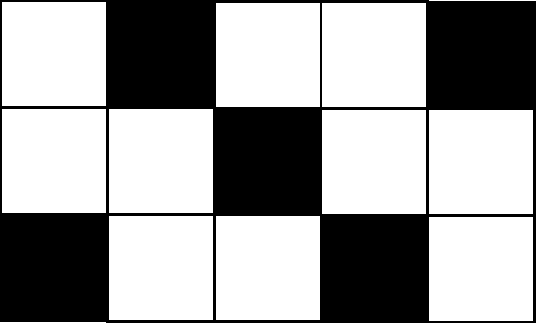
\includegraphics[width=\textwidth]{figures/braet.pdf}
    \end{minipage}
    \hspace*{.1\linewidth}
    \begin{minipage}[h]{0.2\linewidth}
        \centering
        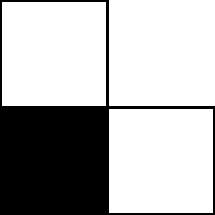
\includegraphics[width=\textwidth]{figures/brik.pdf}
    \end{minipage}
    \vspace*{15pt}
    \caption{Eksempler på et bræt (venstre) og en brik (højre) i Donalds
        puslespil. Bemærk, at brættet i dette eksempel \emph{ikke} har nogen
        løsning.}
\end{figure}

Nogle gange er det dog ikke muligt, at gå puslespillet til at gå op, så
Donald står for at checke om et givent bræt kan lade sig gøre eller ej, og
så smide brættet ud hvis det ikke kan.

Hjælp Donald, ved at lave en $O(mn)$ algoritme, der kan afgøre om et puslespil
kan gå op eller ej.

% Løses med 2SAT: Lav en variabel for om et felt er i samme brik som sin nabo for
% hver nabo. Det giver $O(mn)$ brikker. Lav nu nogle smarte conditions :P
% Kan gøres smartere ved at tælle antallet af hvide og sorte på en speciel måde.


\newpage

\subsection{Den skægge opgave}

% The Collatz conjecture

Her er en funktion for et vilkårligt tal $n$:
\begin{align*}
f(n) = \begin{cases}
n/2 &\text{hvis }n\text{ er lige}\\
3n + 1 &\text{hvis }n\text{ er ulige}\\
\end{cases}
\end{align*}
For eksempel er $f(10) = 5$ og $f(7) = 22$.

Her er en talfølge -- baseret på funktionen $f$ -- der begynder med et
vilkårligt tal $n$:
\begin{align*}
a_i = \begin{cases}
n &\text{når }i = 0\\
f(a_{i - 1}) &\text{når }i > 0\\
\end{cases}
\end{align*}
Hvis vi for eksempel sætter $n = 12$, får vi talfølgen
$a_0 = 12, a_1 = 6, a_2 = 3, a_3 = 10, a_4 = 5, a_5 = 16, a_6 = 8, a_7 = 4, a_8
= 2, a_9 = 1$.  Vi stopper med at vise en talfølge når den når tallet $1$, for
$1$ er et pænt tal, og $f(f(f(1))) = 1$ (vis dette), så den vil alligevel blot
gentage sig.

\textbf{Din opgave:} Bevis eller modbevis følgende formodning:
\begin{quote}
Ligemeget hvilket starttal $n$ der vælges, vil talfølgen altid nå tallet $1$.
\end{quote}

\textbf{\emph{NB: Der udloddes en flaske snaps til den første som kommer op i
baren med en korrekt besvarelse af denne opgave!}}
